%%%%%%%%%%%%%%%%%%%%%%%%%%%%%%%%%%%%%%%%%%%%%%%%%%%%%%%%%%%%%%%%%%% 
%% Introduccion y desarrollo del algoritmo
%%%%%%%%%%%%%%%%%%%%%%%%%%%%%%%%%%%%%%%%%%%%%%%%%%%%%%%%%%%%%%%%%%%


\section{Introduction}
\begin{frame}
  \frametitle{\textbf{Table of Contents}}
  \begin{center}
    {\vspace{-1.5cm}\Large \textbf{Section \thesection}\vspace{0.5cm}}
    \begin{beamercolorbox}[
      sep=8pt,center]{part title}
      \usebeamerfont{part title}
      \textbf{\insertsection}
    \end{beamercolorbox}
  \end{center}
\end{frame}


\begin{frame}
	\frametitle{\textbf{Introduction}}
	\framesubtitle{\secname : \subsecname}
	\begin{block}{\centering \textbf{Objetives}}
		\begin{itemize} \justifying\footnotesize
  			\item Design and implement a 4-parallel pipelined architecture for the Complex Fast Fourier Transform (CFFT) based on the radix-$2^3$ algorithm with 128 points 	using folding transformation and register minimization techniques based on ... .
   			\item Frecuency of implementation: 500MHz. 
  			\item Optimization with CSD\footnote{Canonic Signed Digit} multipliers.
  			\item Test the design with a mixture of two sinusoids using MATLAB.
  			\item Generate power-area-timing report with different
			optimizations. 			
  		\end{itemize}
    \end{block}
\end{frame}



\begin{frame}
	\frametitle{\textbf{Introduction}}
	\framesubtitle{\secname : \subsecname}
	\begin{block}{\centering \textbf{Workflow}}
		\begin{enumerate} \justifying\footnotesize
			\item Obtain the equations that correspond to Butterfly structure of radix-$2^3$ FFT for 8 points.
			\item Apply this idea to design a 2-parallel pipelined architecture radix-$2^3$ 16-points FFT via folding transformation.
			\item Traslate this to a 128-points model.
			\item Elaborate a float-point simulator in Matlab of the 128-points.
			\item Elaborate a synthesizable verilog code HDL and verify the DFT functionality.
			\item Generates power-area-timing report with different optimizations.
		\end{enumerate}
    \end{block}
\end{frame}


\begin{frame}
	\frametitle{\textbf{Introduction}}
    \framesubtitle{\secname : \subsecname}
	\begin{block}{\centering \textbf{Types of pipelined Radix-2 FFT architectures}}
		\begin{enumerate} \justifying\footnotesize
  			\item Feedfoward Multi-Path Delay Commutator (MDC).
  			\item Single-Path Delay Feedback architectures (SDF).
  		\end{enumerate}
		\begin{itemize} \justifying\footnotesize
  			\item Both butterflies and multipliers are in 50\% utilization ... .
  			\item The SDF use registers more efficiently.
  			\item We will focus on the feedfoward MDC asrchitecture.
  		\end{itemize}
    \end{block}

    \vspace{-0.2cm}
    \begin{figure}[!t] \centering
    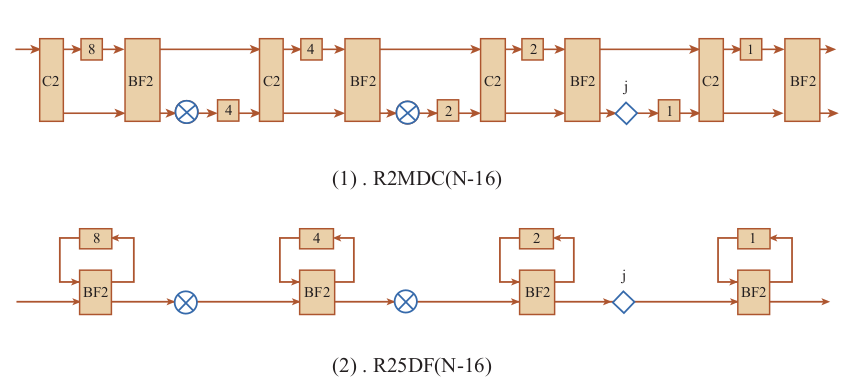
\includegraphics[width=0.70\paperwidth]{./image/types_FFT.png}
    \end{figure}
\end{frame}
